% ==================== 2.3.2.8 金刚石 ====================
\jiegou{2.3.2.8}{金刚石结构}

金刚石结构可视为两套面心立方点阵沿体对角线平移 $(1/4,1/4,1/4)$ 相互穿插而成。这里
用硅演示（$a=5.42$\,\AA 为 Si 的特征值），它与金刚石碳同属金刚石型结构；参数见
表~\ref{tab:diamond}。

\begin{table}[H]
  \centering
  \caption{金刚石结构的建模参数（以 Si 为例）}
  \label{tab:diamond}
  \begin{tabular}{ll}
    \toprule
    项目 & 参数 \\
    \midrule
    空间群 & $F\,d\,\bar3\,m$（No.~227） \\
    晶格常数 & $a=b=c=5.42$\,\AA，$\alpha=\beta=\gamma=90^\circ$ \\
    原子坐标 & Si：$(0,0,0)$（$8a$ 位，另含 $(1/4,1/4,1/4)$ 平移的等效位） \\
    化学式单元数 & $Z=8$ \\
    \bottomrule
  \end{tabular}
\end{table}

\begin{figure}[H]
  \centering
  \subcaptionbox{空间群与晶格常数设置}{%
    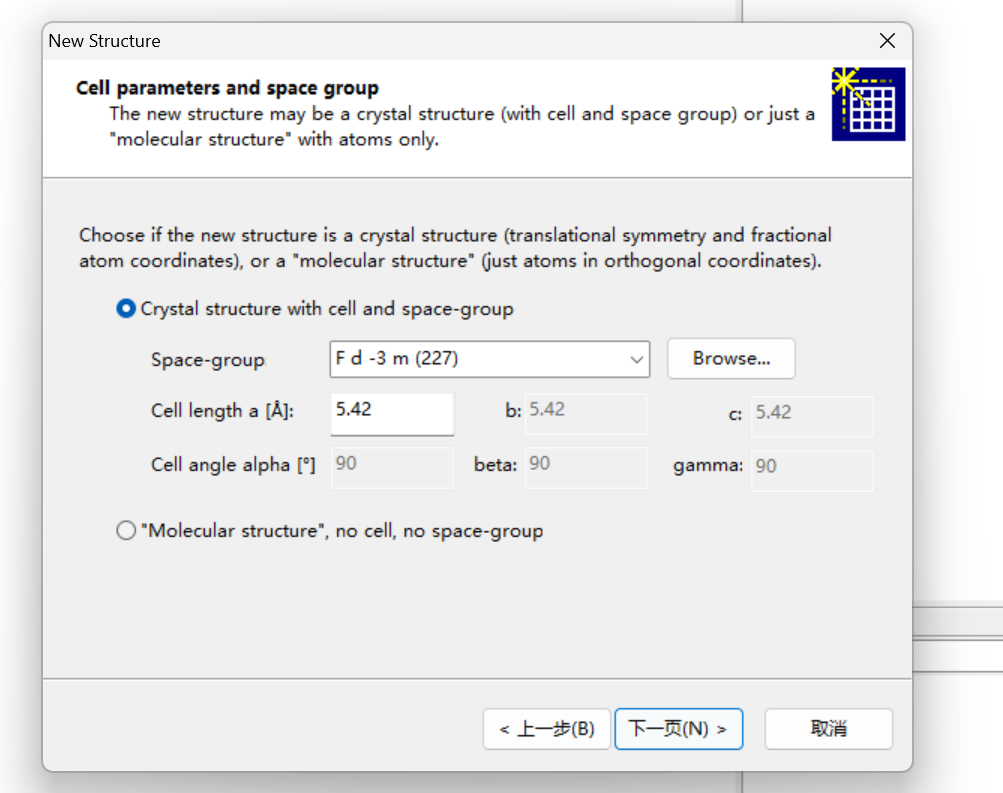
\includegraphics[width=0.44\textwidth]{assets/diamond/a.png}}
  \hfill
  \subcaptionbox{非对称单元原子（Si）添加}{%
    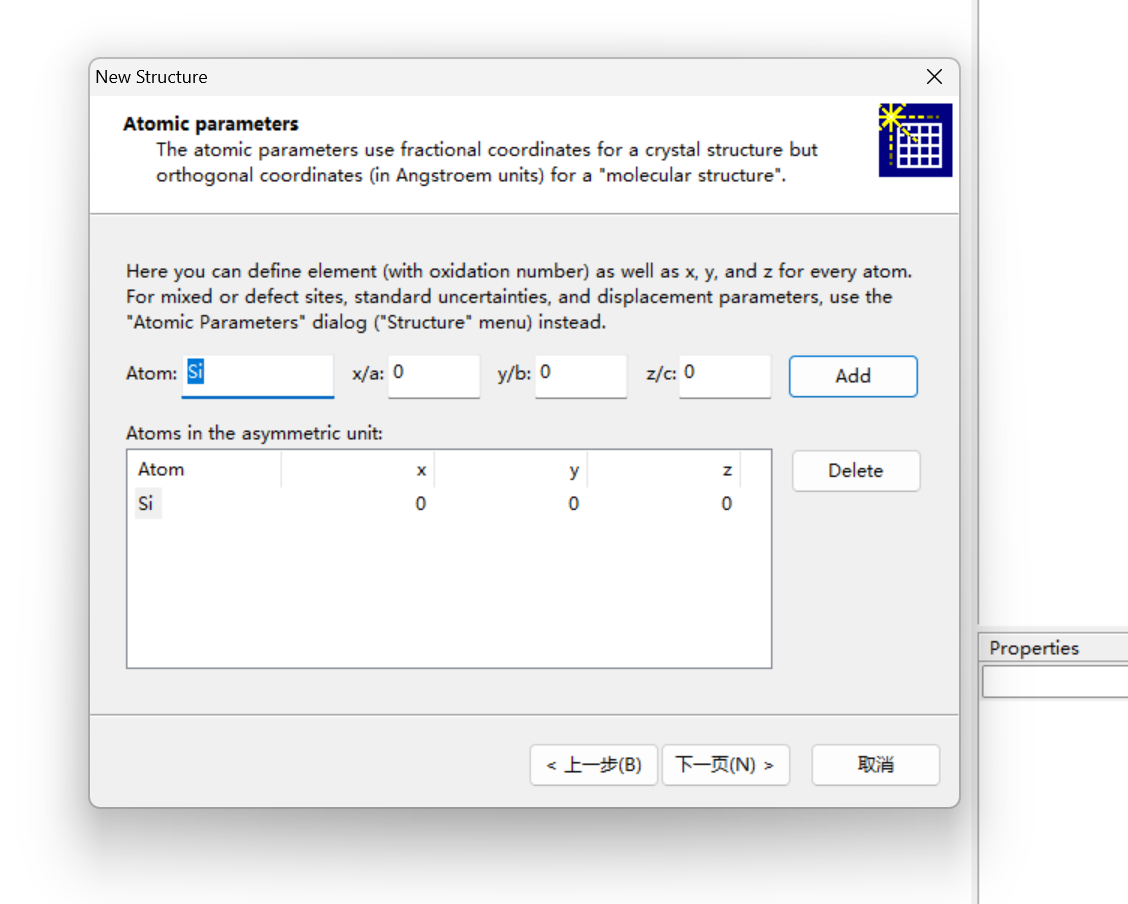
\includegraphics[width=0.44\textwidth]{assets/diamond/b.png}}
  \caption{金刚石结构的参数设置（以 Si 为例）}
  \label{fig:diamond-param}
\end{figure}

\begin{figure}[H]
  \centering
  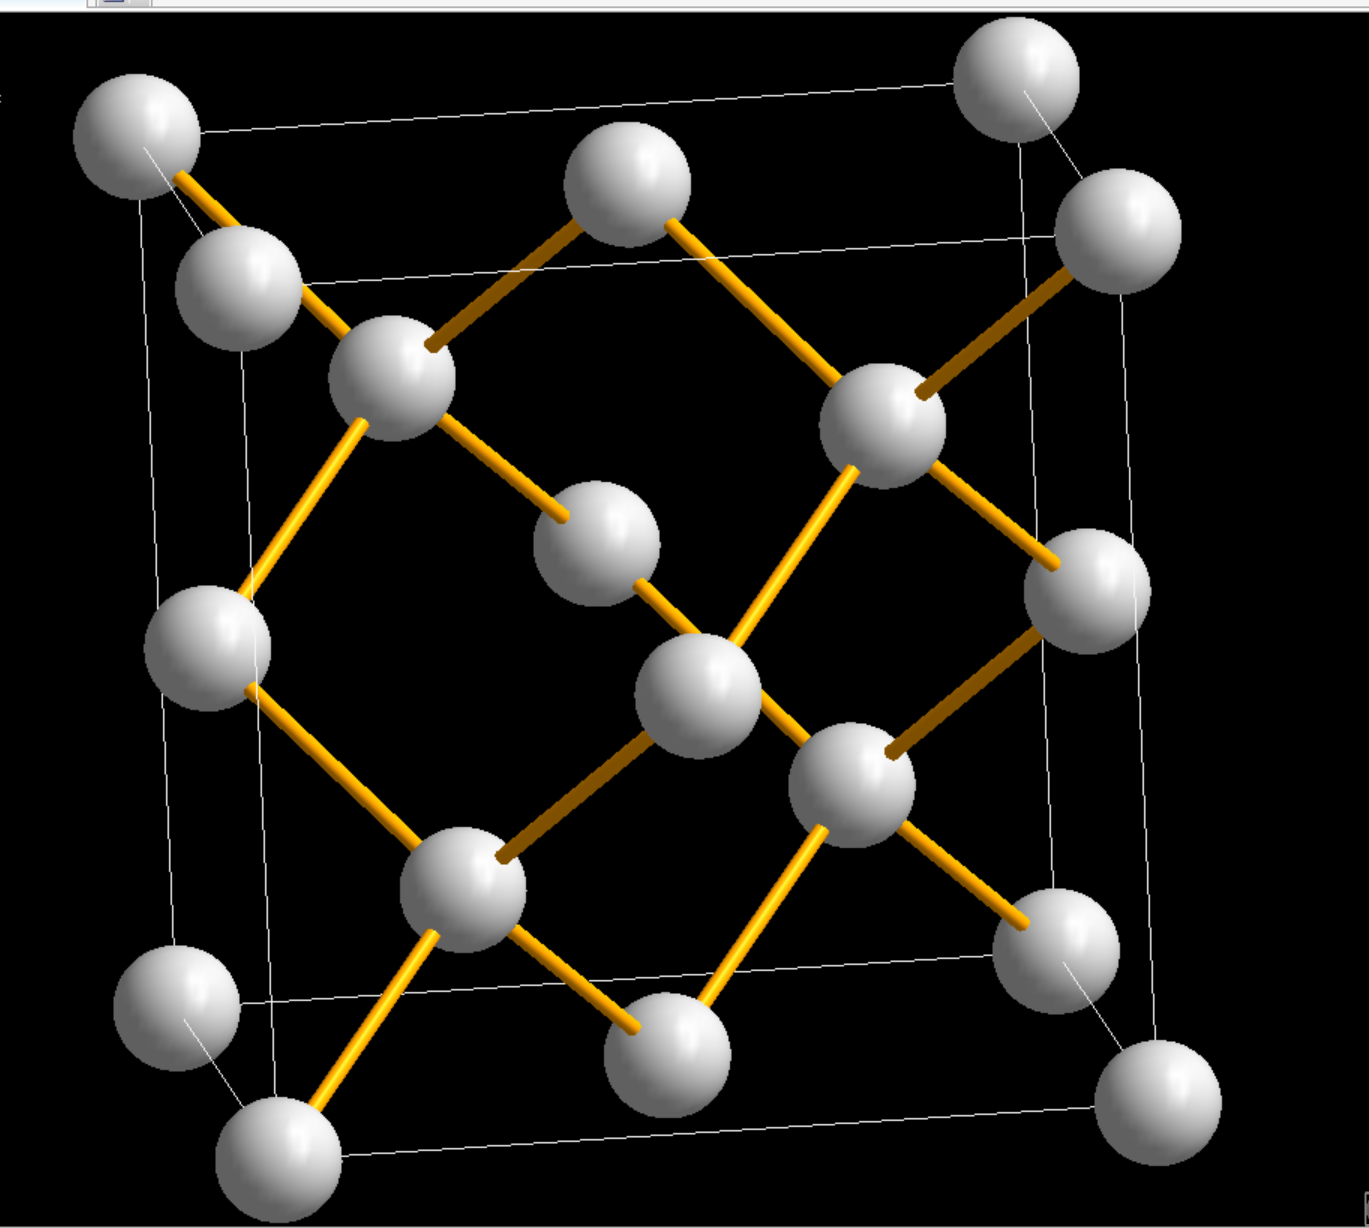
\includegraphics[width=0.5\textwidth]{assets/diamond/c.png}
  \caption{金刚石结构的晶体结构模型（以 Si 为例）}
  \label{fig:diamond-model}
\end{figure}

\begin{figure}[H]
  \centering
  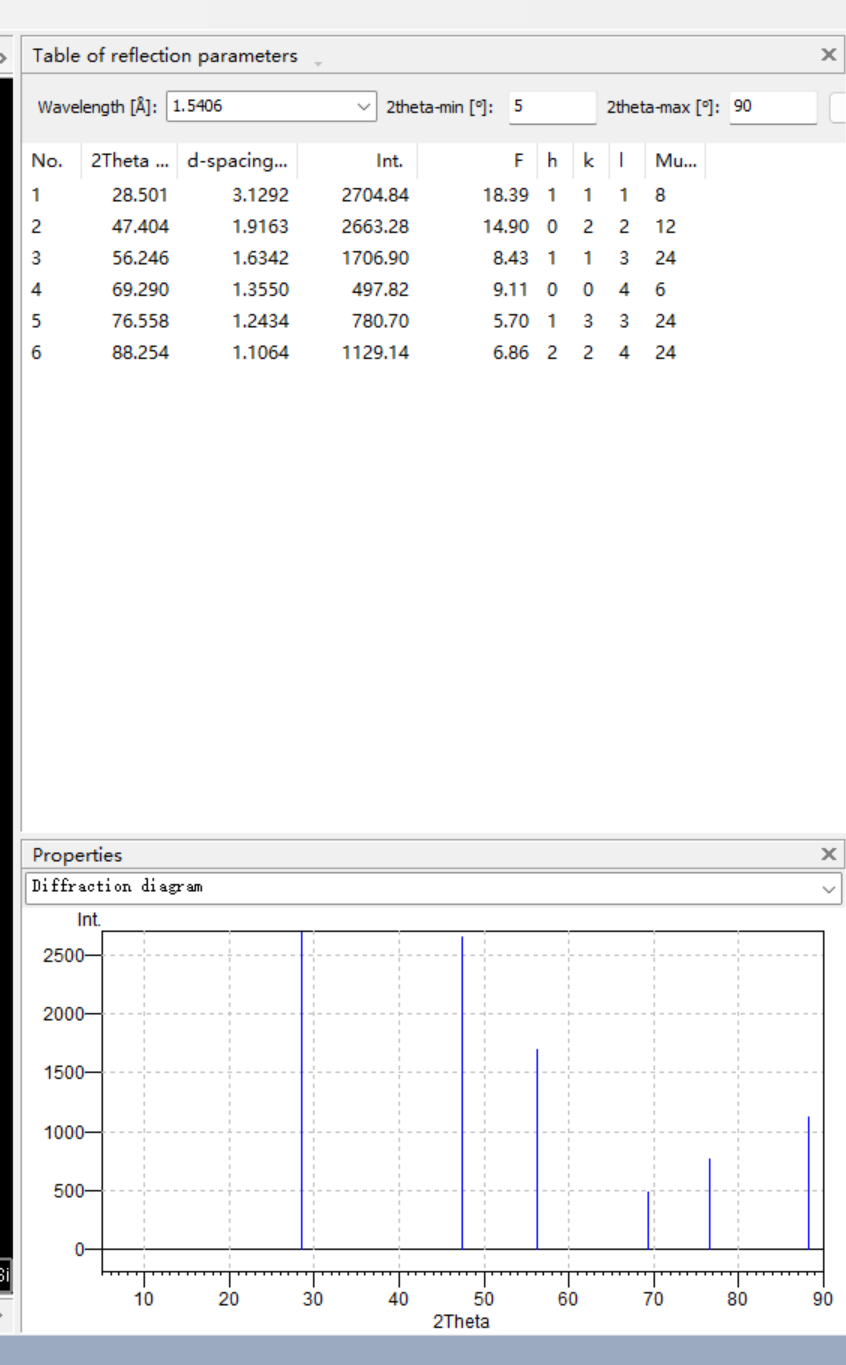
\includegraphics[width=0.4\textwidth]{assets/diamond/d.png}
  \caption{Diamond 模拟的金刚石结构粉末衍射图}
  \label{fig:diamond-xrd}
\end{figure}

\begin{figure}[H]
  \centering
  \subcaptionbox{晶面视图}{%
    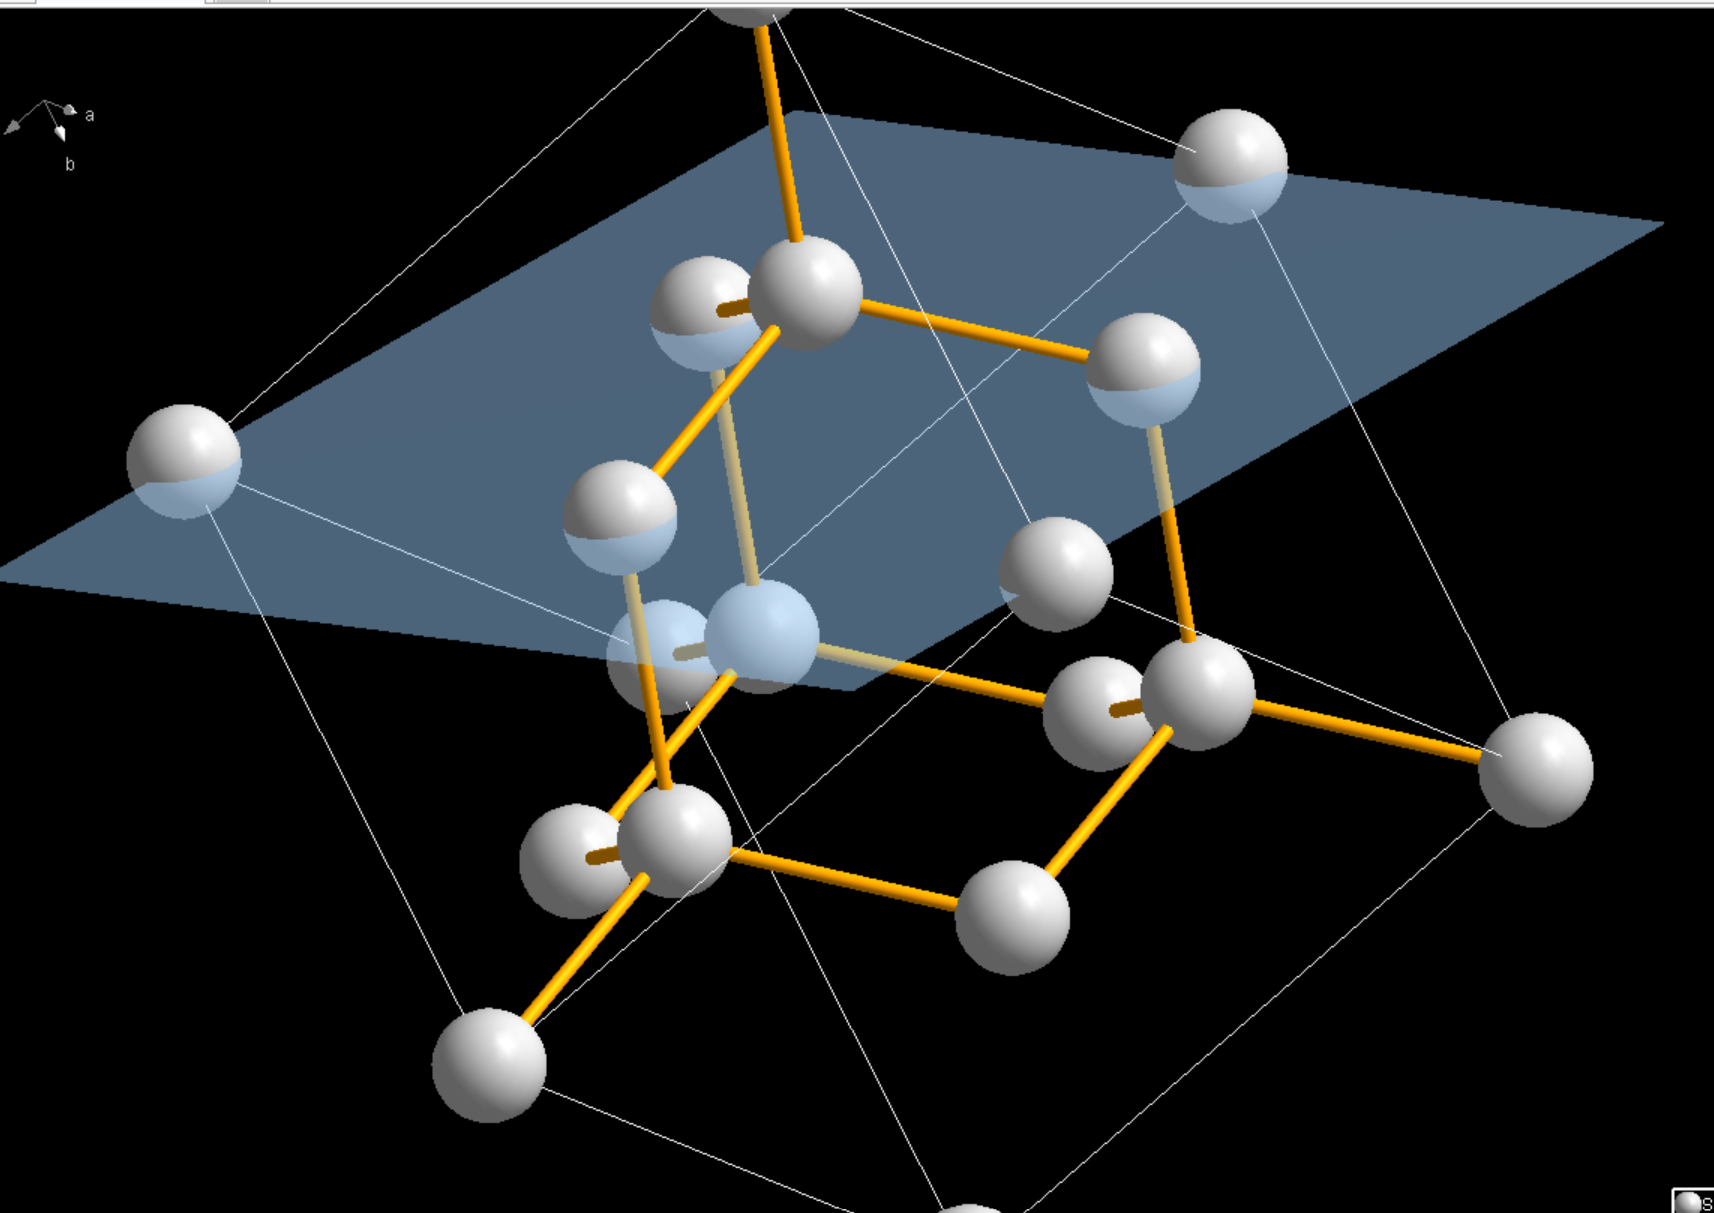
\includegraphics[width=0.44\textwidth]{assets/diamond/e.png}}
  \hfill
  \subcaptionbox{四面体配位（配位数 4）}{%
    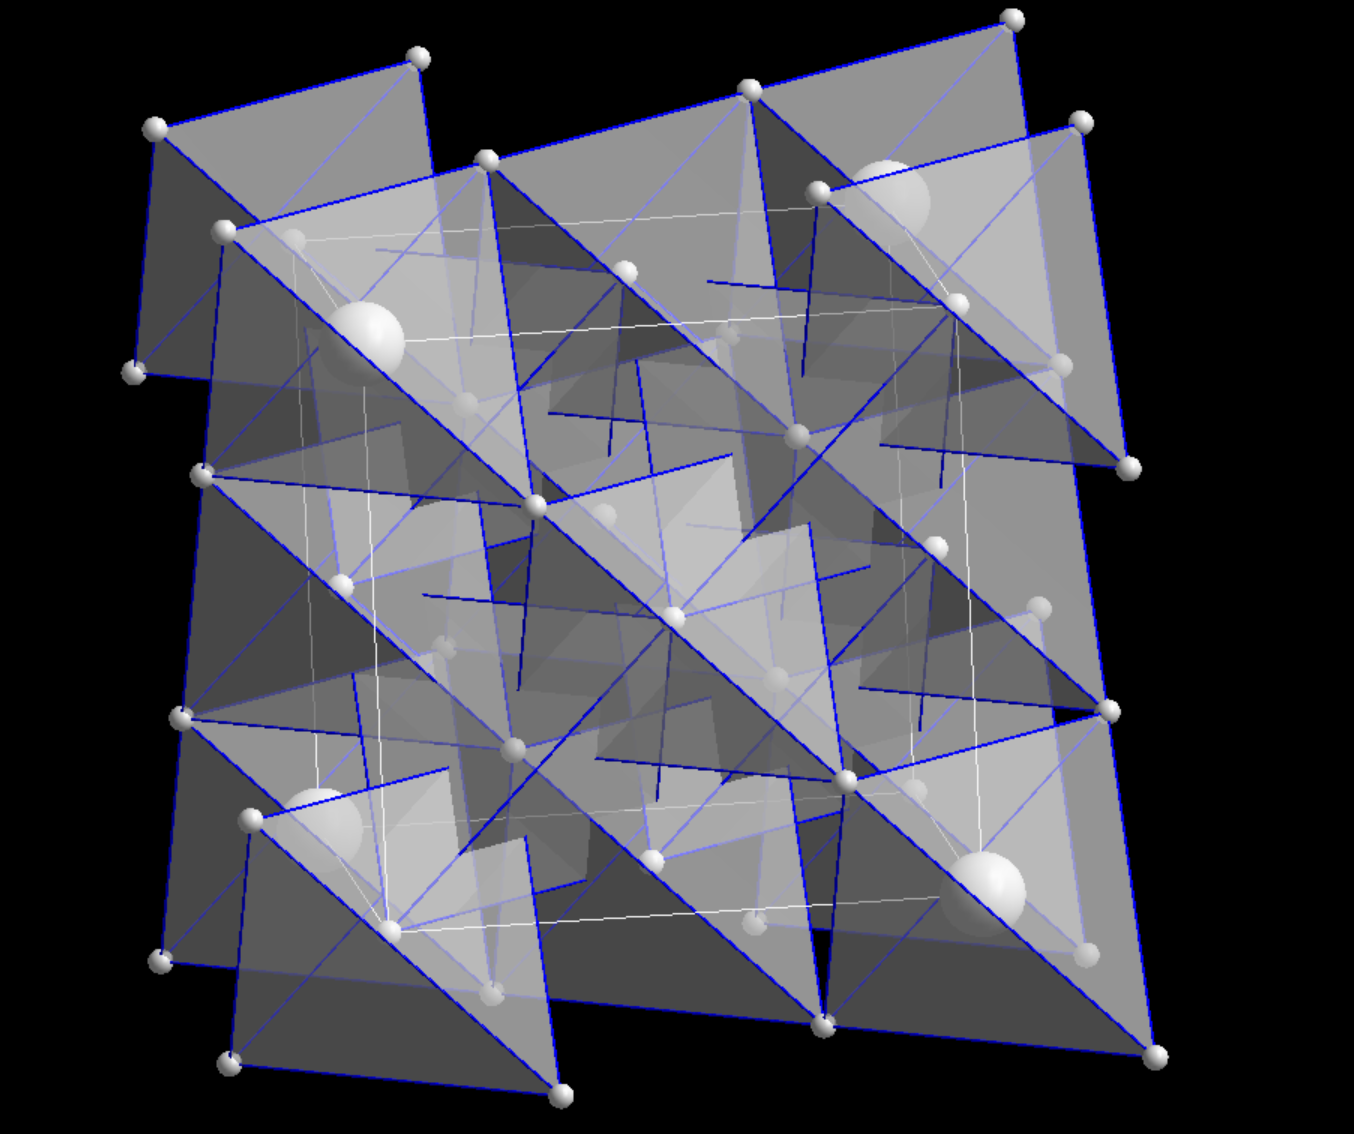
\includegraphics[width=0.44\textwidth]{assets/diamond/f.png}}
  \caption{金刚石结构的晶面与四面体配位}
  \label{fig:diamond-plane}
\end{figure}

\textbf{结构要点。}晶胞内共 8 个原子：4 个在一套 FCC 点阵（顶点与面心）上，另 4 个在
沿体对角线平移 $(1/4,1/4,1/4)$ 的第二套 FCC 点阵上。每个原子与 4 个最近邻以 $sp^3$
杂化轨道成键，构成正四面体配位（图~\ref{fig:diamond-plane}(b)），键角
$109.47^\circ$；最近邻距离（键长）为体对角线的 $1/4$：
\begin{equation}
  d=\frac{\sqrt{3}}{4}a=\frac{\sqrt{3}}{4}\times5.42\approx2.35\ \text{\AA}
\end{equation}
把原子视作沿体对角线相切的刚球（$2r=\sqrt{3}a/4$），堆积因子为
\begin{equation}
  \eta=\frac{8\times\frac{4}{3}\pi\left(\frac{\sqrt{3}}{8}a\right)^3}{a^3}
    =\frac{\pi\sqrt{3}}{16}\approx0.3401
\end{equation}
远低于 FCC 的 $0.7405$。堆积因子的偏小说明结构中存在大量未被占据的空间，这与金刚石
较低的密度（约 $3.5$ g/cm$^3$）相符；其极高的硬度则来自 C--C 共价键的键能与方向性，
两者并不矛盾。$F\,d\,\bar3\,m$ 中的 $d$ 即金刚石滑移面（镜面反映加 $1/4$ 平移），
它把两套 FCC 亚格子联系了起来。

金刚石型结构是共价晶体的典型代表：金刚石（C）是自然界最硬的物质，同型的 Si、Ge 是
最重要的半导体材料，$\alpha$-Sn（灰锡）也属此结构。
